% ==============================================================================
% Section 4.2: Geographic Concentration (RQ1)
% ==============================================================================
\subsection{Geographic Concentration (RQ1)}
\label{sec:concentration_results}
Across all \nmonths{} months, disappearances are extremely geographically concentrated regardless of outcome status.
The Gini coefficient exceeds 0.91 for every status in every month of the study period (Table~\ref{tab:concentration}).
Located Dead is the most concentrated, with a mean Gini of 0.979 (range: 0.963 to 0.993), followed by Located Alive (mean: 0.955), Not Located (mean: 0.946), and Total (mean: 0.935).

This concentration substantially exceeds standard criminological benchmarks.
\citet{weisburd_2015}'s ``law of crime concentration'' posits that approximately 50\% of crime concentrates in 4 to 6\% of micro-geographic units (street segments).
At the municipal level, concentration is even more pronounced: in \referencemonth{}, 50\% of Not Located registrations concentrate in just 42 municipalities (1.7\% of \nmunis{}), and 50\% of Located Dead registrations in 22 municipalities (0.9\%). Even the least concentrated status, Total, requires only 48 municipalities (1.9\%) to account for half of all registrations.


\begin{figure}[htbp]
  \centering
  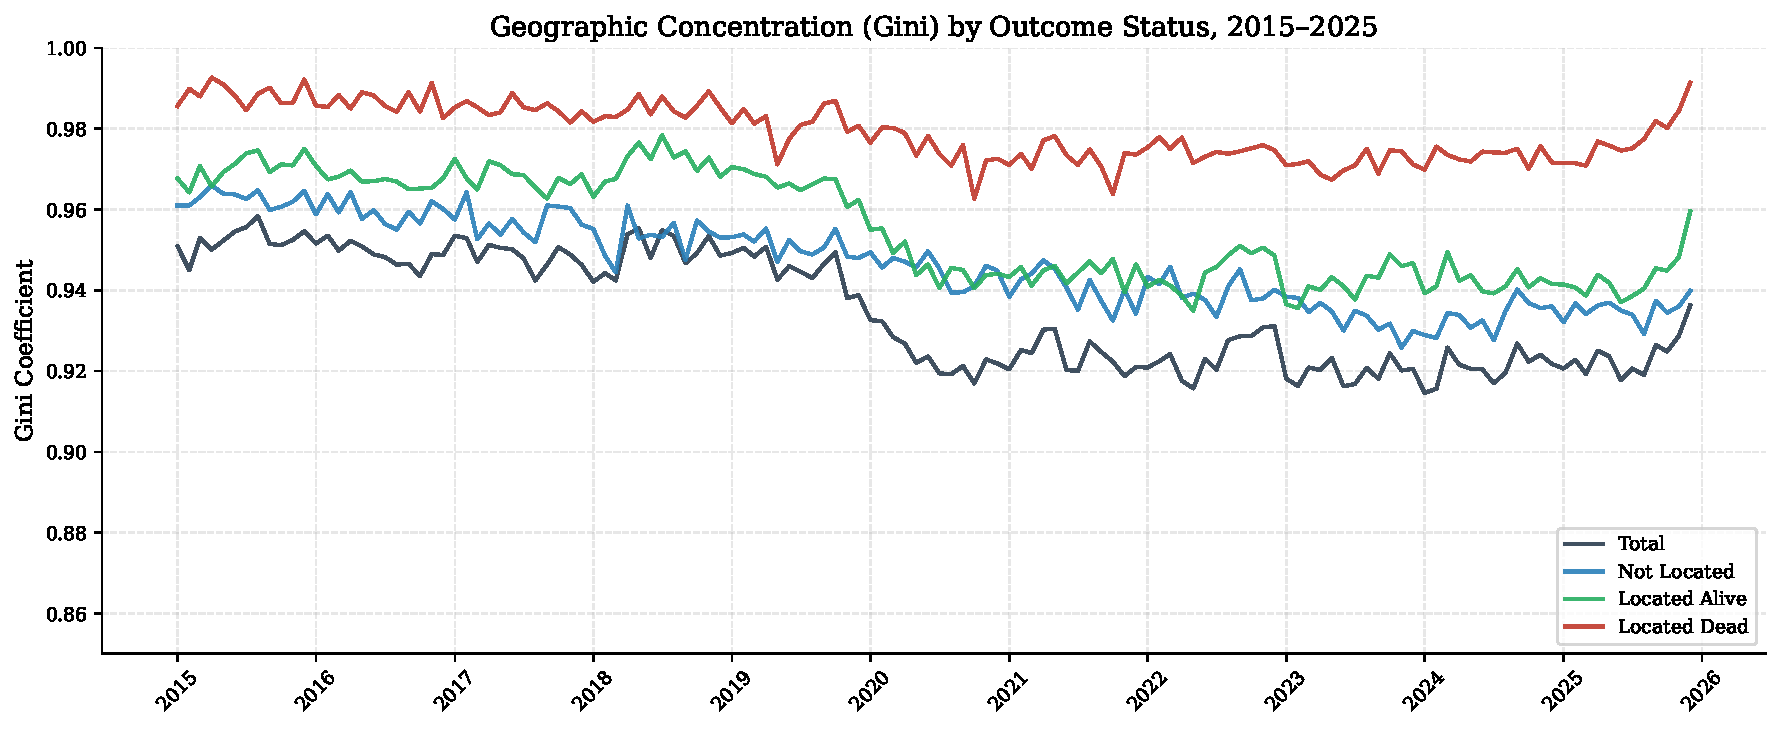
\includegraphics[width=\textwidth]{figures/fig2_gini_time_series.pdf}
  \caption{Gini coefficient of monthly case count distributions by outcome status, \studyperiod{}.
           OLS trend slopes (Gini units per year) annotated.
           Dashed horizontal line indicates Gini = 0.90 reference.}
  \label{fig:gini}
\end{figure}

Despite the extreme levels, all four Gini series exhibit statistically significant negative trends (Figure~\ref{fig:gini}; Table~\ref{tab:concentration}): Total $-0.0038$/yr ($p < 0.001$), Not Located $-0.0032$/yr ($p < 0.001$), Located Alive $-0.0035$/yr ($p < 0.001$), and Located Dead $-0.0017$/yr ($p < 0.001$).
This gradual deconcentration reflects the geographic spread of disappearances into municipalities that previously recorded zero cases: in \bookendstart{}, 88.8\% of municipalities recorded zero Total cases; by \referencemonth{}, this had fallen to 77.0\%.
The deconcentration trend is substantively modest: after a decade of geographic diffusion, concentration remains far above the Weisburd benchmark.

\begin{table}[htbp]
\centering
\caption{Gini coefficient by outcome status, \nmonths{} monthly observations, \studyperiod{}.}\label{tab:concentration}
\begin{tabular}{lrrrr}
  \toprule
  \textbf{Status} & \textbf{Mean} & \textbf{Min} & \textbf{Max} & \textbf{Trend}\tnote{a} \\
  \midrule
  Total         & 0.935 & 0.915 & 0.958 & $-$0.004*** \\
  Not Located   & 0.946 & 0.926 & 0.966 & $-$0.003*** \\
  Located Alive & 0.955 & 0.935 & 0.978 & $-$0.004*** \\
  Located Dead  & 0.979 & 0.963 & 0.993 & $-$0.002*** \\
  \bottomrule
\end{tabular}
\begin{tablenotes}
\small
\item[a] OLS slope per year ($\times$12), 132 monthly observations. $^{***}p<0.001$.
\end{tablenotes}
\end{table}